\documentclass[preprint,12pt]{elsarticle}
\usepackage{amsmath,amssymb,mathtools}
\usepackage{booktabs}
\usepackage{graphicx}
\usepackage{array}
\usepackage{tabularx}
\setlength{\emergencystretch}{3em}
\usepackage{hyperref}
\hypersetup{hidelinks}
\renewcommand{\thefigure}{S\arabic{figure}}
\renewcommand{\thetable}{S\arabic{table}}
\graphicspath{{../figures/}}
\newcommand{\one}{\mathbf 1}
\newcommand{\pos}[1]{[#1]_+}
\newcommand{\algname}{SC-WDP}

\begin{document}
\begin{frontmatter}
\title{Supplementary Material for ``Sparse Convex Optimization for Winner Determination: Approximation Guarantees and Anytime Dominance''}
\author{Angshul Majumdar}
\address{Indraprastha Institute of Information Technology Delhi, New Delhi 110020, India}
\begin{abstract}
This supplement reports synthetic numerical diagnostics targeted only at results that are specific to the proposed sparse-convex WDP framework. It does not repeat the CATS benchmark study and does not compare against external solvers. The tests examine the constructive weighted-support equivalence, the uniform rejection repair, the certified outer-bracket contraction, the finite-tolerance exact-recovery mechanism for uniquely integral LP optima, and the retained-incumbent/gap-certificate logic. The numerical results are supporting evidence rather than substitutes for the proofs in the main manuscript. All data, plots, and the Python scripts that regenerate them are included in the accompanying repository.
\end{abstract}
\end{frontmatter}

\section{Scope and reproducibility}
The purpose of this supplement is deliberately narrow. The main manuscript already contains the proofs. Here we construct small synthetic WDP instances for which the exact LP and, when required, the exact binary WDP can be solved independently, and then check the theorem-specific invariants numerically. No external baseline is used in this supplement.

All experiments use random seed \texttt{20261012}. Linear programs and the small binary reference problems are solved by the HiGHS back end exposed through SciPy. The synthetic implementation follows the formulas of the main manuscript in double precision. Therefore statements such as ``verified'' below mean verified numerically to the stated floating-point accuracy; the rigorous certification result remains the real-arithmetic theorem in the main paper.

Two synthetic instance families are used. The \emph{overlap} family draws nonempty bid bundles uniformly up to a stated maximum cardinality and assigns continuous positive values
\[
  v_j=1+2|S_j|+U_j,\qquad U_j\sim\operatorname{Unif}(0,5),
\]
with a final pass ensuring that each item appears in at least two bids. The \emph{partition} family has three singleton bids per item and a deliberately separated unique highest-valued bid in every item group. The latter gives well-conditioned uniquely integral LP instances for the full outer-bracket trace.

\section{Constructive exact weighted-support equivalence}
The exact continuous weighted-support theorem states that any feasible fractional rejection vector can be thresholded at zero to a binary feasible rejection vector without changing weighted support. We tested the constructive map itself rather than solving a redundant second combinatorial problem.

For each of 25 overlap instances with six items and 14 bids, we generated 20 feasible fractional rejection vectors by taking convex combinations of two feasible binary rejection vectors obtained from independently randomized greedy allocations. For each point $z$, we formed
\[
 \widehat z_j=\mathbf 1_{\{z_j>0\}}.
\]
Across all 500 trials, the thresholded point remained feasible and the weighted-support objective was unchanged to machine precision. Table~\ref{tab:support-repair} summarizes this test together with the repair experiment described next.

\section{Uniform rejection repair}
The main manuscript defines
\[
 r=\pos{b-Az},\qquad
 \theta(z)=\max_i\frac{r_i}{1+r_i},\qquad
 \mathcal R(z)=z+\theta(z)(\one-z),
\]
and proves both $A\mathcal R(z)\ge b$ and $\theta(z)\le\|r\|_\infty$.

We sampled 2,000 independent box points $z\in[0,1]^m$ over the same 25 overlap instances. Every repaired point satisfied the covering constraints to within $1.8\times10^{-15}$ numerical roundoff. No sample violated $\theta(z)\le\|r\|_\infty$. Figure~\ref{fig:repair} shows all 2,000 pairs against the theorem boundary.

\begin{table}[t]
\centering
\caption{Synthetic checks of the constructive weighted-support map and the uniform rejection repair. Numerical feasibility margins below zero are roundoff at the $10^{-15}$ level.}
\label{tab:support-repair}
\small
\begin{tabularx}{\linewidth}{@{}Xrr@{}}
\toprule
Check & Samples & Worst observed discrepancy \\
\midrule
Weighted-support objective after thresholding & 500 & $0$ \\
Thresholded feasibility margin & 500 & $0$ minimum \\
Repair inequality $\theta-\|r\|_\infty$ & 2,000 & $-3.67\times10^{-1}$ maximum \\
Post-repair feasibility margin & 2,000 & $-1.78\times10^{-15}$ minimum \\
\bottomrule
\end{tabularx}
\end{table}

\begin{figure}[t]
\centering
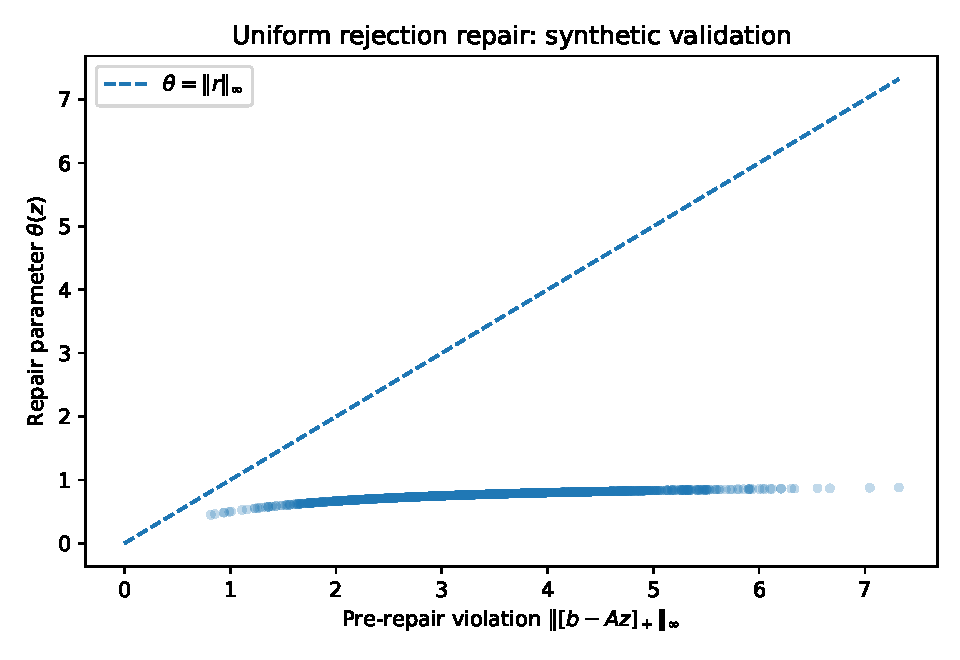
\includegraphics[width=0.78\linewidth]{figS1_repair.pdf}
\caption{Synthetic validation of the uniform rejection repair. Every point lies below the theorem boundary $\theta(z)=\|[b-Az]_+\|_\infty$.}
\label{fig:repair}
\end{figure}

\section{Certified outer-bracket contraction}
We next exercised the complete numerical outer solver, including SPG inner iterations, the residual-dual lower event, the repair-based upper event, and warm starts. Ten independently generated partition instances were used, each with five items and three bids per item. The exact rejection-LP optimum $P^\star$ was solved independently and was used only to audit the bracket after every completed outer iteration.

For every recorded iteration and every instance,
\[
 L_J\le P^\star\le U_J
\]
held numerically. Moreover,
\[
 \frac{U_J-L_J}{W}\le\left(\frac23\right)^J
\]
held in every row of the generated data; the largest observed excess over the theoretical envelope was $2.22\times10^{-16}$. Figure~\ref{fig:bracket} plots the ten trajectories. Upper events often contract the interval by more than the worst-case factor, which explains why several traces fall substantially below the envelope.

\begin{figure}[t]
\centering
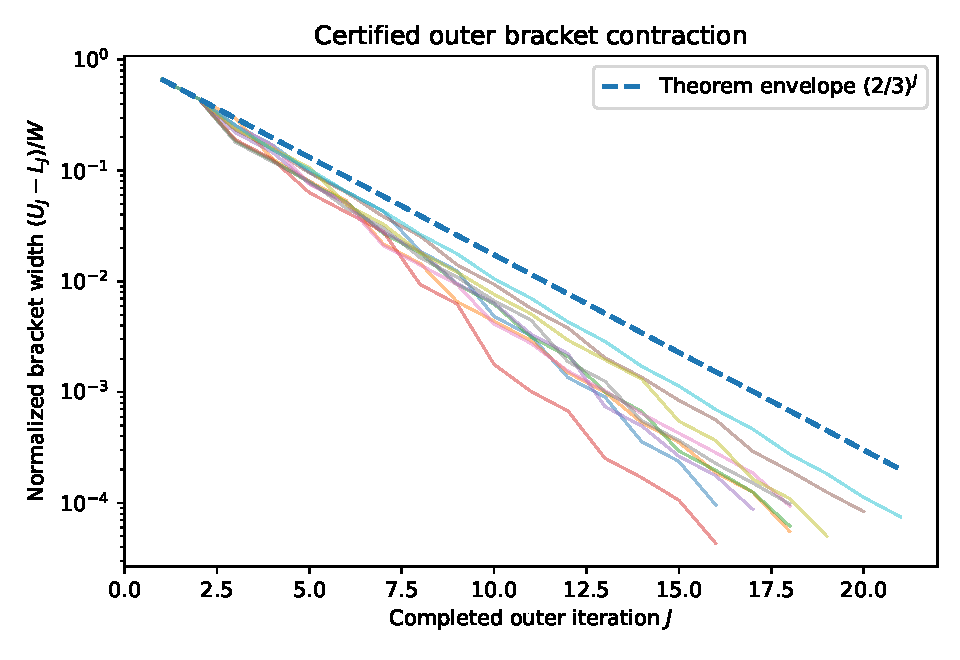
\includegraphics[width=0.80\linewidth]{figS2_bracket.pdf}
\caption{Normalized bracket widths for ten synthetic runs of the complete outer solver. The dashed curve is the theorem envelope $(2/3)^J$. All independently checked LP optima remained inside the corresponding numerical brackets.}
\label{fig:bracket}
\end{figure}

\section{Finite-tolerance exact recovery}
The finite-tolerance exact-recovery theorem is specific to instances whose natural LP has a unique integral optimum. Its proof introduces the objective-separation constant
\[
 \varepsilon_0=\gamma
 =\min_{z\in\mathcal F:\,\|z-z^{\rm LP}\|_\infty\ge1/4}
   \bigl(v^\top z-P^\star\bigr)>0.
\]
For a binary $z^{\rm LP}$, this quantity can be computed by $2m$ auxiliary LPs, one for each coordinate side of the $\ell_\infty$ neighborhood. We generated overlap instances with five items and ten bids until 30 instances with an integral LP optimum and positive $\gamma$ were obtained. Continuous random bid values make an exact objective tie a probability-zero event; the auxiliary LP separation additionally confirms strict positive separation at the $1/4$ boundary.

For each instance and each ratio $\rho=\varepsilon/\varepsilon_0$, we then solved an adversarial auxiliary problem that maximizes
\[
 \|z-z^{\rm LP}\|_\infty
\]
over all LP-feasible $z$ satisfying $v^\top z\le P^\star+\varepsilon$. Because $z^{\rm LP}$ is binary, this maximization reduces to coordinatewise LPs. Thus Figure~\ref{fig:recovery-geometry} does not show a favorable random witness: it shows the worst feasible witness under the specified objective tolerance.

For every tested $\rho<1$, the worst feasible distance remained strictly below $1/4$; the largest value was $0.2475$ at $\rho=0.99$. At $\rho=1$, the boundary $1/4$ becomes attainable, exactly matching the separation definition used in the proof. Fractional-priority recovery was exact on all 30 instances for every tested $\rho<1$. Once the theorem condition was deliberately violated, the guarantee disappeared: the exact-recovery rate was $76.7\%$ at $\rho=2$ and $0\%$ at $\rho=4$; see Figure~\ref{fig:recovery-rate}. These latter points are not a sharpness theorem, but they show that the finite-tolerance condition is operational rather than vacuous.

\begin{figure}[t]
\centering
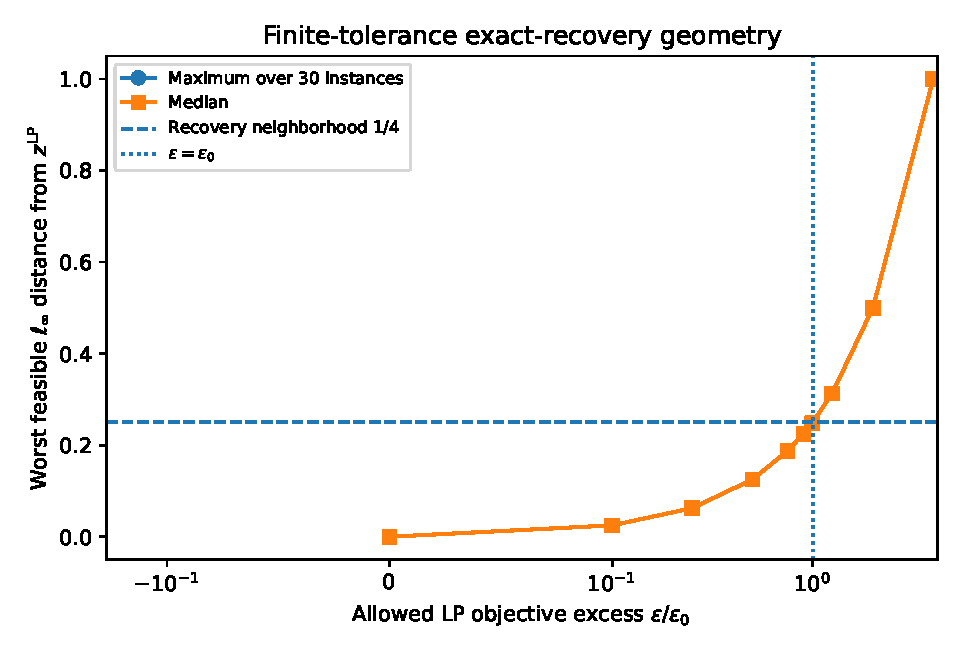
\includegraphics[width=0.80\linewidth]{figS3_exact_recovery.pdf}
\caption{Worst feasible $\ell_\infty$ distance from the unique integral LP optimum under an allowed objective excess $\varepsilon$. The horizontal line is the $1/4$ ordering neighborhood used by the proof; the vertical line marks $\varepsilon=\varepsilon_0$.}
\label{fig:recovery-geometry}
\end{figure}

\begin{figure}[t]
\centering
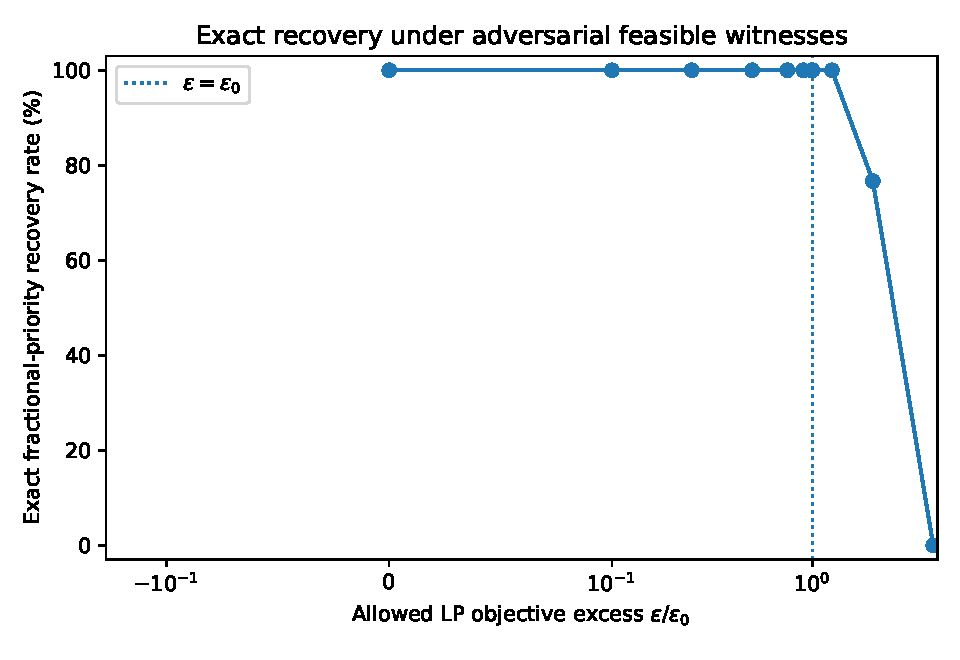
\includegraphics[width=0.80\linewidth]{figS3b_recovery_rate.pdf}
\caption{Exact fractional-priority recovery from the adversarial feasible witnesses used in Figure~\ref{fig:recovery-geometry}. All 30 instances recover exactly throughout the theorem regime $\varepsilon<\varepsilon_0$.}
\label{fig:recovery-rate}
\end{figure}

\section{Retained-incumbent dominance and the online gap certificate}
The internal anytime theorem is a retention statement: after the descending-value safeguard is available, the reported incumbent is the maximum over that safeguard and every completed convex-guided recovery. The gap corollary simultaneously provides the online upper bound
\[
 G(x^{\rm best})
 \le 1-\frac{v^\top x^{\rm best}}{W-L}.
\]
We illustrate both mechanisms on a fixed-seed overlapping instance with five items and ten bids for which convex-guided recovery strictly improves the safeguard. The exact binary optimum is solved independently only for plotting the true gap.

At checkpoint zero the descending-value safeguard has a $22.60\%$ exact-solution gap. The first completed outer iteration produces the exact binary allocation, after which the retained incumbent remains exact. The online certificate is necessarily more conservative: it starts at $66.24\%$ and contracts monotonically as the lower bracket endpoint increases, reaching $0.0423\%$ by the final plotted iteration. At every checkpoint the computable certificate remains above the independently evaluated true gap. Figure~\ref{fig:gap-certificate} also shows the frozen safeguard gap, making the internal anytime dominance visible directly. Zero true gaps are plotted at $10^{-6}$ only to permit logarithmic display.

\begin{figure}[t]
\centering
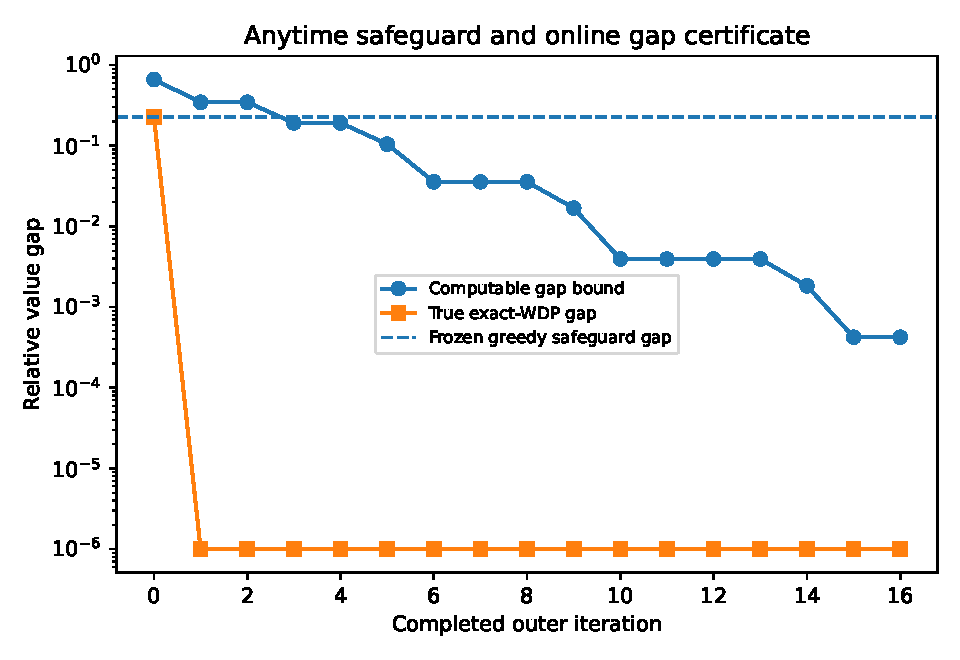
\includegraphics[width=0.80\linewidth]{figS4_gap_certificate.pdf}
\caption{Representative synthetic trace of the retained incumbent and computable exact-WDP gap certificate. The incumbent improves over the frozen safeguard and is never discarded; the online certificate remains a valid upper bound on the independently evaluated true gap and tightens as the bracket contracts.}
\label{fig:gap-certificate}
\end{figure}

\section{What these experiments do and do not establish}
The synthetic experiments are deliberately theorem-facing. They confirm that the constructive maps and inequalities behave exactly as predicted on generated instances, that the complete numerical bracket respects the theoretical contraction envelope on the audited runs, that the finite-tolerance recovery neighborhood appears at the separation constant used in the proof, and that the retained-incumbent and online-gap logic are numerically consistent with independently solved small WDPs.

They do not replace any proof in the main manuscript, do not establish asymptotic complexity empirically, and do not make claims about superiority over an external solver. In particular, the outer-bracket theorem is an exact real-arithmetic statement, whereas the reference implementation in this repository uses IEEE double precision. The purpose of releasing the scripts and raw CSV files is to make these numerical diagnostics inspectable and exactly reproducible.

\end{document}
